% Model report generated by SolverMapp.
% Compile with: pdflatex, bibtex, pdflatex, pdflatex (references.bib is written by the first run).
\begin{filecontents*}[overwrite]{references.bib}
@misc{ref,
  note   = {Chenciner, A., Montgomery, R. (2000). A remarkable periodic solution of the three-body problem in the case of equal masses. Annals of Mathematics, 152, 881-901.},
  key    = {Chenciner, A., Montgomery, R. (2000). A }
}
\end{filecontents*}
\documentclass[11pt,a4paper]{article}
\usepackage[T1]{fontenc}
\usepackage[utf8]{inputenc}
\usepackage{lmodern}
\usepackage{amsmath,amssymb}
\usepackage{booktabs,longtable}
\usepackage{siunitx}
\usepackage{algorithm}
\usepackage{algpseudocode}
\usepackage{tikz}
\usetikzlibrary{positioning,shapes.geometric,shapes.misc,arrows.meta}
\usepackage{adjustbox}
\usepackage[hidelinks]{hyperref}

\title{N-body problem in index notation (figure-eight, N = 3)}
\author{}
\date{\today}

\begin{document}
\maketitle

The model consists of 3 equations in 7 variables: 4 inputs, 2 state variables, 0 intermediate variables and 1 output. It is solved in 2 steps (Algorithm~\ref{alg:solution}).

\section{Nomenclature}
\begin{longtable}{@{}l p{0.48\linewidth} l l@{}}
  \toprule
  Symbol & Description & Unit & Value \\
  \midrule
  \endhead
  \bottomrule
  \endfoot
  \multicolumn{4}{@{}l}{\textit{Inputs}} \\
  $t$ & Time & \si{s} & \num{0} \\
  $G$ & Gravitational constant (normalised) & \si{m^{3}/(kg.s^{2}} & \num{1} \\
  $m$ & Masses & \si{kg} & \num{1} \\
  $N$ & Number of bodies & -- & \num{3} \\
  \addlinespace
  \multicolumn{4}{@{}l}{\textit{State variables}} \\
  $\mathbf{v}$ & Velocities, one row per body & \si{m/s} & 0.466203685, 0.43236573; 0.466203685, 0.43236573; -0.93240737, -0.86473146 \\
  $\mathbf{r}$ & Positions, one row per body & \si{m} & 0.97000436, -0.24308753; -0.97000436, 0.24308753; 0, 0 \\
  \addlinespace
  \multicolumn{4}{@{}l}{\textit{Outputs}} \\
  $E$ & Total energy & \si{J} &  \\
\end{longtable}

\section{Governing equations}

\subsection{Positions}
Source: \cite{ref}, Eq.~(1).
\begin{equation}
  \frac{d\mathbf{r}_i}{dt} = \mathbf{v}_i
  \label{eq:positions}
\end{equation}
\noindent where

\noindent\begin{tabular}{@{\quad}l@{\quad}p{0.7\linewidth}@{}}
  $\mathbf{r}$ & Positions, one row per body, \si{m} \\
  $\mathbf{v}$ & Velocities, one row per body, \si{m/s} \\
  $t$ & Time, \si{s} \\
\end{tabular}

\noindent Holds for every $i = 1, \dots, N$. Integrated over $t$ from $0$ to $6.32591398$ with the classical fourth-order Runge–Kutta method in 2000 steps, starting from the start value of $\mathbf{r}$, together with Eq.~\eqref{eq:velocities}. The solution is saved every 10 steps.

\subsection{Velocities}
Source: \cite{ref}, Eq.~(2).
\begin{equation}
  \frac{d\mathbf{v}_i}{dt} = \sum_{j \ne i} G m_j \frac{\mathbf{r}_j - \mathbf{r}_i}{\|\mathbf{r}_j - \mathbf{r}_i\|^3}
  \label{eq:velocities}
\end{equation}
\noindent where

\noindent\begin{tabular}{@{\quad}l@{\quad}p{0.7\linewidth}@{}}
  $\mathbf{v}$ & Velocities, one row per body, \si{m/s} \\
  $G$ & Gravitational constant (normalised), \si{m^{3}/(kg.s^{2}} \\
  $m$ & Masses, \si{kg} \\
  $\mathbf{r}$ & Positions, one row per body, \si{m} \\
  $t$ & Time, \si{s} \\
\end{tabular}

\noindent Holds for every $i = 1, \dots, N$. Integrated over $t$ from $0$ to $6.32591398$ with the classical fourth-order Runge–Kutta method in 2000 steps, starting from the start value of $\mathbf{v}$, together with Eq.~\eqref{eq:positions}. The solution is saved every 10 steps.

\subsection{Total energy}
Source: \cite{ref}, Eq.~(3).
\begin{equation}
  E = \sum_i \frac{1}{2} m_i \|\mathbf{v}_i\|^2 - \sum_{i<j} \frac{G m_i m_j}{\|\mathbf{r}_i - \mathbf{r}_j\|}
  \label{eq:total-energy}
\end{equation}
\noindent where

\noindent\begin{tabular}{@{\quad}l@{\quad}p{0.7\linewidth}@{}}
  $E$ & Total energy, \si{J} \\
  $m$ & Masses, \si{kg} \\
  $\mathbf{v}$ & Velocities, one row per body, \si{m/s} \\
  $G$ & Gravitational constant (normalised), \si{m^{3}/(kg.s^{2}} \\
  $\mathbf{r}$ & Positions, one row per body, \si{m} \\
\end{tabular}


\section{Solution algorithm}
\begin{algorithm}[htbp]
  \caption{Solution procedure}\label{alg:solution}
  \begin{algorithmic}[1]
    \State Set the inputs $G$, $m$ and $N$
    \State Set the start values $\mathbf{v}$ and $\mathbf{r}$
    \For{$t = 0$ to $6.32591398$ in 2000 steps} \Comment{RK4}
      \State Advance $\mathbf{r}$ and $\mathbf{v}$ by one RK4 step of Eq.~\eqref{eq:positions} and Eq.~\eqref{eq:velocities}
    \EndFor
    \State Compute $E$ from Eq.~\eqref{eq:total-energy}
  \end{algorithmic}
\end{algorithm}

Figure~\ref{fig:flowchart} shows the same procedure as a flowchart.

\begin{figure}[htbp]
  \centering
  \begin{adjustbox}{max width=\linewidth, max totalheight=0.9\textheight}
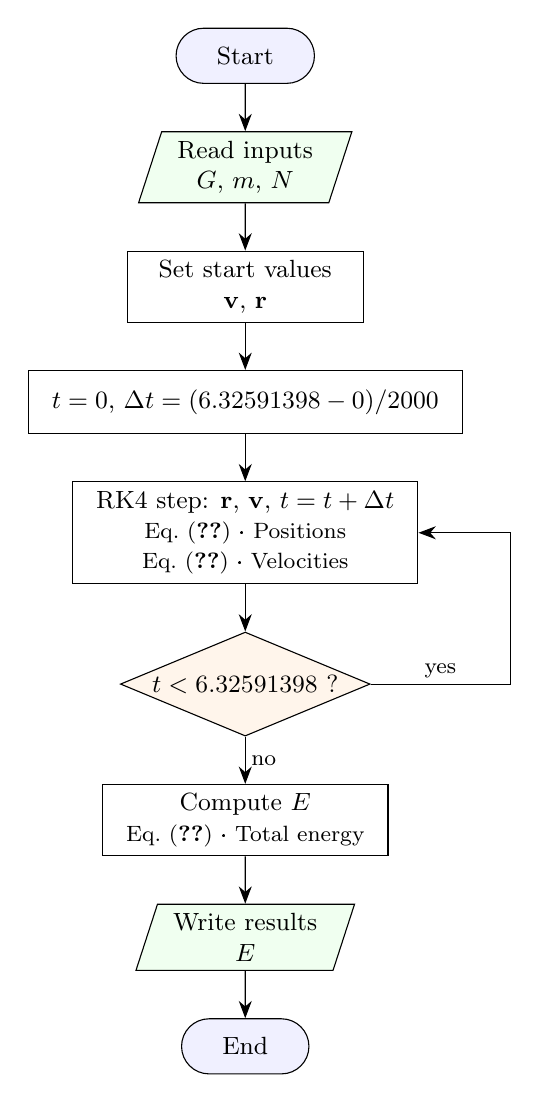
\begin{tikzpicture}[
  node distance=6mm, >={Stealth[length=2.2mm]}, font=\small,
  every node/.style={align=center},
  term/.style={draw, rounded rectangle, minimum height=7mm, inner xsep=5mm, fill=blue!6},
  io/.style={draw, trapezium, trapezium left angle=72, trapezium right angle=108, trapezium stretches body, minimum height=8mm, inner xsep=2mm, fill=green!6},
  proc/.style={draw, rectangle, minimum height=8mm, minimum width=30mm, inner xsep=3mm},
  dec/.style={draw, diamond, aspect=2.4, inner sep=1pt, fill=orange!8},
  lbl/.style={font=\footnotesize, inner sep=2pt}]
  \node[term] (n1) {Start};
  \node[io, below=of n1] (n2) {Read inputs \\ $G$, $m$, $N$};
  \node[proc, below=of n2] (n3) {Set start values \\ $\mathbf{v}$, $\mathbf{r}$};
  \node[proc, below=of n3] (n4) {$t = 0$, $\Delta t = (6.32591398 - 0) / 2000$};
  \node[proc, below=of n4] (n5) {RK4 step: $\mathbf{r}$, $\mathbf{v}$, $t = t + \Delta t$ \\ {\footnotesize Eq.~\eqref{eq:positions} \textperiodcentered{} Positions} \\ {\footnotesize Eq.~\eqref{eq:velocities} \textperiodcentered{} Velocities}};
  \node[dec, below=of n5] (n6) {$t < 6.32591398$ ?};
  \node[proc, below=of n6] (n7) {Compute $E$ \\ {\footnotesize Eq.~\eqref{eq:total-energy} \textperiodcentered{} Total energy}};
  \node[io, below=of n7] (n8) {Write results \\ $E$};
  \node[term, below=of n8] (n9) {End};
  \coordinate (E) at (current bounding box.east);
  \coordinate (L0) at ([xshift=6mm]E);
  \draw[->] (n1) -- (n2);
  \draw[->] (n2) -- (n3);
  \draw[->] (n3) -- (n4);
  \draw[->] (n4) -- (n5);
  \draw[->] (n5) -- (n6);
  \draw[->] (n6) -- node[lbl, right] {no} (n7);
  \draw[->] (n7) -- (n8);
  \draw[->] (n8) -- (n9);
  \draw[->] (n6.east) -- node[lbl, above] {yes} (n6.east -| L0) |- (n5.east);
\end{tikzpicture}
  \end{adjustbox}
  \caption{Flowchart of the solution procedure}\label{fig:flowchart}
\end{figure}

\bibliographystyle{plain}
\bibliography{references}

\end{document}